\documentclass{article}
\usepackage{mainPoly}

\title{Suites arithmétiques}
\date{}
\author{Terminale STMG 2}

\begin{document}
\maketitle
\section{Termes d'une suite arithmétique}
\begin{tcolorbox}
\begin{definition}[Rappel]
Une suite arithmétique est une suite numérique $\left(u_n\right)_{n \in \N}$ définie par son \textbf{premier terme} $u_0$ et un nombre $r$ appelé la \textbf{raison}, tel que chaque terme $u_n$ pour $n > 0$ est obtenu en ajoutant $r$ au terme précédent :
\begin{equation*}
u_n = u_{n-1} + r
\end{equation*} 
\end{definition}
\end{tcolorbox}
\begin{example}
\begin{itemize}
\item La suite
\begin{equation*}
0; 2; 4; 6; 8; 10; \dots
\end{equation*}
est la suite de premier terme $0$ et de raison $2$.
\begin{center}
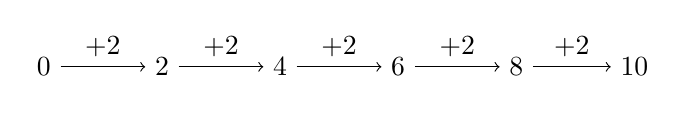
\begin{tikzpicture}
\node (A) at (0,0) {$0$};
\node (B) at (1.5,0) {$2$};
\node (C) at (3,0) {$4$};
\node (D) at (4.5,0) {$6$};
\node (E) at (6,0) {$8$};
\node (F) at (7.5,0) {$10$};

\draw[->, bend left] (A) -- (B) node[midway, above] {$+2$}; 
\draw[->, bend left] (B) -- (C) node[midway, above] {$+2$};
\draw[->, bend left] (C) -- (D) node[midway, above] {$+2$};
\draw[->, bend left] (D) -- (E) node[midway, above] {$+2$};
\draw[->, bend left] (E) -- (F) node[midway, above] {$+2$};
\end{tikzpicture}
\end{center}
\item La suite 
\begin{equation*}
10; 9; 8; 7; 6; 5; \dots    
\end{equation*}
est la suite de premier terme $10$ et de raison $-1$.
\item La suite $1;2;4;7;11;\dots$ n'est pas une suite arithmétique. En effet,
\begin{center}
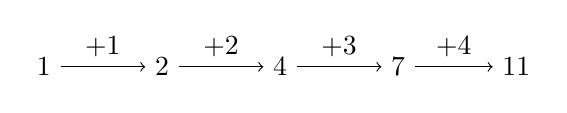
\begin{tikzpicture}
\node (A) at (0,0) {$1$};    
\node (B) at (1.5,0) {$2$};
\node (C) at (3,0) {$4$};
\node (D) at (4.5,0) {$7$};
\node (E) at (6,0) {$11$};

\draw[->] (A) -- (B) node[midway, above] {$+1$};
\draw[->] (B) -- (C) node[midway, above] {$+2$};
\draw[->] (C) -- (D) node[midway, above] {$+3$};
\draw[->] (D) -- (E) node[midway, above] {$+4$};
\end{tikzpicture}
\end{center}
\end{itemize}
\end{example}
\begin{remark}
Une suite arithmétique est constante (tous ses termes sont égaux) si et seulement si sa raison est égale à $0$.
\end{remark}
\begin{proposition}
Soit $\left(u_n\right)_{n \in \N}$ une suite arithmétique de raison $r$. Alors, son $n$\ieme terme est donné par la formule
\begin{equation*}
u_0 + n \times r
\end{equation*}
\end{proposition}
\begin{example}
\hfill
\begin{enumerate}[label=\emph{\alph*)}]
\item Donner le $5$\ieme terme de la suite arithmétique de premier terme $3,5$ et de raison $3$ : \answersline
\item Donner le $10$\ieme terme de la suite arithmétique de premier terme $12$ et de raison $-5$ : \answersline 
\end{enumerate}
\end{example}
\begin{tcolorbox}
En résumé, il y a deux types d'écriture pour le $n$\ieme terme d'une suite arithmétique :
\begin{itemize}
\item La formule de récurrence $u_n = u_{n - 1} + r$. Pour vérifier qu'une suite est arithmétique, on vérifie qu'on obtient chaque terme en ajoutant $r$ au terme précédent.
\item La formule explicite $u_n = u_0 + n \times r$. On l'utilise une fois qu'on sait qu'une suite arithmétique, pour calculer directement le $n$\ieme terme.
\end{itemize} 
\end{tcolorbox}
\end{document}